\chapter{Testing Scenarios, Results, and Discussions}
\label{chap:results}

\section{Experimental Scenario Matrix and Benchmark Setup}
\label{sec:res_matrix}
Nghiên cứu triển khai hệ thống 14 kịch bản thực nghiệm đối chứng có kiểm soát chặt chẽ (từ E1 đến E6, bao gồm khảo sát sâu dải siêu tham số $\mu$) trên cùng một môi trường phần cứng và cấu hình siêu tham số đồng nhất:
\begin{itemize}
    \item Số vòng giao tiếp liên đoàn: $T = 10$ rounds.
    \item Số epoch huấn luyện cục bộ: $E = 2$ epochs/round.
    \item Kích thước batch cục bộ: $B_{\text{size}} = 64$.
    \item Tốc độ học: $\eta = 10^{-3}$ với bộ tối ưu AdamW.
    \item Hệ số phạt FedProx: $\mu = 0.05$.
    \item Tập kiểm định đánh giá: $100\%$ kịch bản đều được đánh giá độc lập trên cùng tập \textbf{Global Holdout Test Set ($30\%$ Data)} gồm đúng $1,534,918$ mẫu.
\end{itemize}

\section{Master Benchmark Results and Synthesis}
\label{sec:res_master}
Bảng \ref{tab:master_results} trình bày toàn bộ kết quả đo kiểm thực nghiệm thu được từ 10 kịch bản đã hoàn thành trong hệ sinh thái của đề tài.

\begin{table}[H]
\centering
\caption{Master benchmark results of the FL-IoT-IDS system on CICIoT2023.}
\label{tab:master_results}
\small
\begin{tabularx}{\textwidth}{>{\raggedright\arraybackslash}X c c c c c c}
\toprule
\textbf{Experimental Scenario} & \textbf{Accuracy} & \textbf{Macro-F1} & \textbf{Web-based} & \textbf{Brute-force} & \textbf{Comm Cost} & \textbf{Drift} \\
& \textbf{(\%)} & \textbf{(\%)} & \textbf{Recall (\%)} & \textbf{Recall (\%)} & \textbf{(MB)} & \textbf{L2 Norm} \\
\midrule
\multicolumn{7}{l}{\textit{Group E1: Centralized Upper-Bound Baseline}} \\
E1: Centralized Baseline & 78.69 & 63.70 & \textbf{52.41} & \textbf{53.36} & 0.00 & 0.00 \\
\midrule
\multicolumn{7}{l}{\textit{Group E2: Homogeneous Benchmark (IID, $K=5$)}} \\
E2: FedAvg (IID, $K=5$) & \textbf{84.52} & \textbf{67.75} & \textbf{0.85} & \textbf{20.75} & 5.30 & 9.63 \\
E2: FedProx ($\mu=0.05$, IID, $K=5$) & 80.09 & 59.06 & 0.00 & 0.00 & 5.30 & \textbf{0.52} \\
\midrule
\multicolumn{7}{l}{\textit{Group E3: Mild Non-IID Skew ($\alpha=1.0, K=5$)}} \\
E3: FedAvg ($\alpha=1.0, K=5$) & 84.42 & 67.62 & 0.39 & 21.54 & 5.30 & 10.75 \\
E3: FedProx ($\mu=0.05, \alpha=1.0, K=5$) & 77.41 & 55.45 & 0.00 & 0.00 & 5.30 & 0.56 \\
\midrule
\multicolumn{7}{l}{\textit{Group E4: Moderate Non-IID Skew ($\alpha=0.5, K=5$)}} \\
E4: FedAvg ($\alpha=0.5, K=5$) & 81.94 & 64.73 & 1.44 & 18.37 & 5.30 & 13.30 \\
E4: FedProx ($\mu=0.05, \alpha=0.5, K=5$) & 75.99 & 53.01 & 0.00 & 0.00 & 5.30 & 0.60 \\
\midrule
\multicolumn{7}{l}{\textit{Group E5: Severe Non-IID Skew ($\alpha=0.1, K=5$) \& $\mu$ Sensitivity Sweep}} \\
E5: FedAvg ($\alpha=0.1, K=5$) & 74.84 & 53.25 & 0.00 & 0.00 & 5.30 & 22.39 \\
E5: FedProx ($\mu=0.001, \alpha=0.1, K=5$) & \textbf{77.75} & \textbf{57.42} & 0.00 & \textbf{12.38} & 5.30 & 2.06 \\
E5: FedProx ($\mu=0.01, \alpha=0.1, K=5$) & 74.71 & 51.75 & 0.00 & 0.00 & 5.30 & 0.98 \\
E5: FedProx ($\mu=0.025, \alpha=0.1, K=5$) & 74.02 & 50.32 & 0.00 & 0.00 & 5.30 & 0.73 \\
E5: FedProx ($\mu=0.05, \alpha=0.1, K=5$) & 70.12 & 43.01 & 0.00 & 0.00 & 5.30 & \textbf{0.65} \\
\midrule
\multicolumn{7}{l}{\textit{Group E6: Client Scalability Benchmark (IID)}} \\
E6: FedAvg (IID, $K=7$) & 84.54 & 67.82 & 0.63 & 21.10 & 7.42 & 8.42 \\
E6: FedAvg (IID, $K=10$) & 84.41 & 67.28 & 0.39 & 19.21 & \textbf{10.60} & 7.25 \\
\bottomrule
\end{tabularx}
\end{table}

\section{In-depth Analysis of Core Scientific Findings}
\label{sec:res_findings}

\subsection{Finding 1: Empirical Counter-Evidence on Minority Class Collapse (Negative Finding)}
Đối chiếu trực diện giữa kịch bản tập trung (E1) và các kịch bản phân tán (E2--E6) mang lại một phát hiện khoa học mang tính bước ngoặt:
\begin{itemize}
    \item \textbf{Năng lực nội tại của kiến trúc mô hình:} Khi huấn luyện tập trung (E1) với toàn bộ dữ liệu, mô hình \texttt{TabularIoTMLP} đạt tỷ lệ phát hiện (Recall) lên tới $\mathbf{52.41\%}$ trên lớp \texttt{Web-based} và $\mathbf{53.36\%}$ trên lớp \texttt{Brute-force} (xem Hình \ref{fig:recall_e1_centralized}). Điều này chứng minh rằng kiến trúc nơ-ron MLP 3 tầng hoàn toàn có đủ dung lượng biểu diễn để trích xuất các đặc trưng phân loại của các lớp tấn công thiểu số.
    \item \textbf{Sự sụp đổ do cơ chế tổng hợp phân tán (FedAvg):} Khi phân tán sang môi trường liên đoàn FedAvg, tỷ lệ Recall của \texttt{Web-based} sụt giảm thảm hại xuống $1.66\%$ ($K=5$) và tiếp tục rơi xuống $0.39\%$ khi mở rộng lên $K=10$ clients. Nguyên nhân toán học nằm ở công thức (\ref{eq:fedavg_agg}): lớp Web-based chỉ chiếm $0.49\%$ dữ liệu, khiến gradient của các trạm chứa lớp này bị "pha loãng" và triệt tiêu hoàn toàn bởi hàng trăm nghìn mẫu của các lớp DDoS/DoS khi tính trung bình gia quyền $n_k/N$.
    \item \textbf{Hiệu ứng phong tỏa tính dẻo của FedProx (Loss of Local Plasticity):} Đáng chú ý, ở tất cả các kịch bản sử dụng FedProx với $\mu=0.05$, Recall của cả Web-based và Brute-force đều rơi thẳng về $\mathbf{0.00\%}$. Số hạng phạt $\frac{\mu}{2}\|\mathbf{w} - \mathbf{w}_t\|_2^2$ đã cưỡng chế vector tham số client không được dịch chuyển xa khỏi mô hình toàn cục, vô tình dập tắt nỗ lực di chuyển gradient để học các mẫu hiếm.
\end{itemize}

\begin{figure}[H]
    \centering
    \begin{subfigure}[b]{0.48\textwidth}
        \centering
        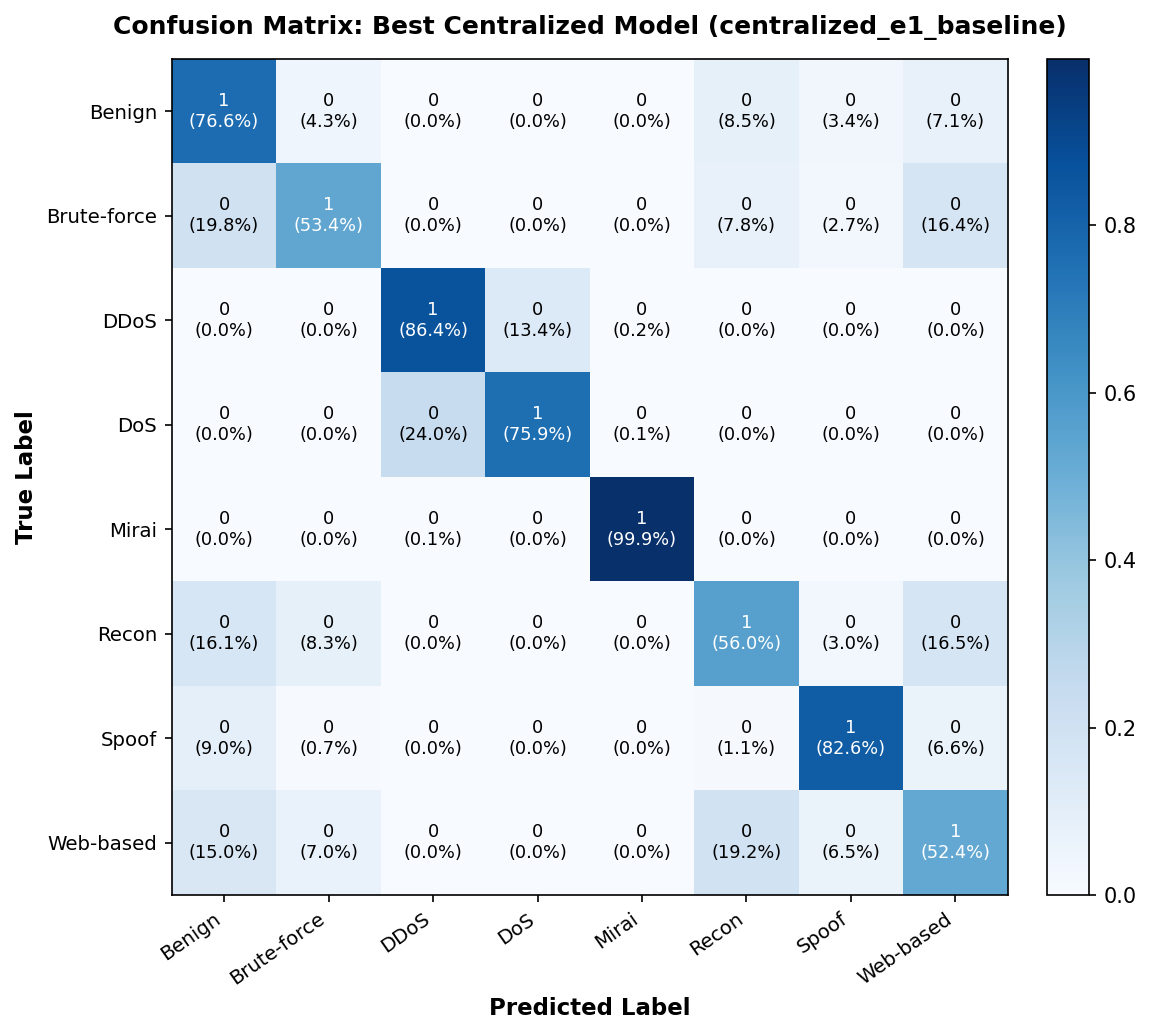
\includegraphics[width=\textwidth]{figures/cm_e1_centralized.png}
        \caption{Normalized confusion matrix: E1 Centralized Baseline.}
        \label{fig:cm_e1_centralized}
    \end{subfigure}
    \hfill
    \begin{subfigure}[b]{0.48\textwidth}
        \centering
        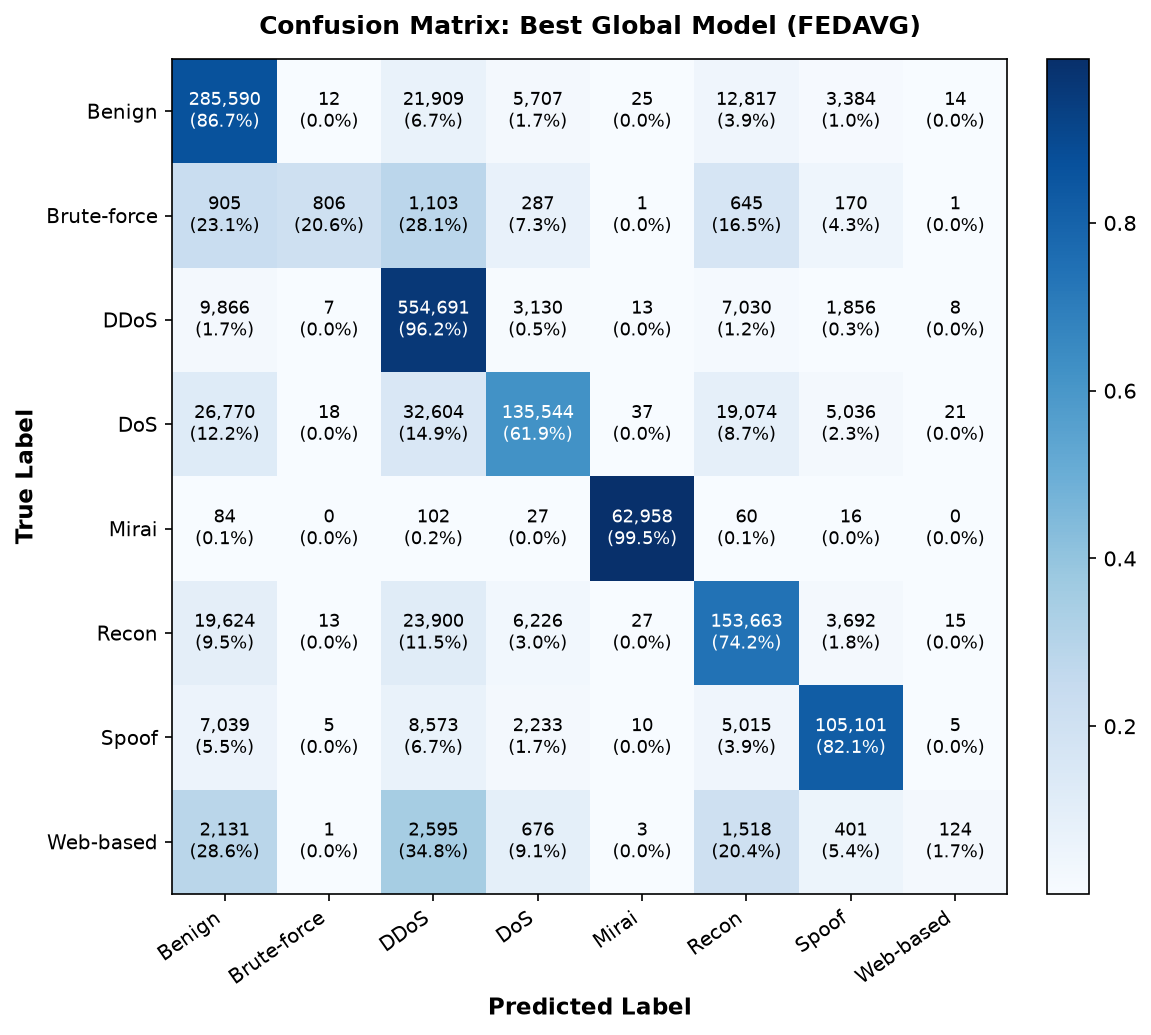
\includegraphics[width=\textwidth]{figures/cm_e2_fedavg.png}
        \caption{Normalized confusion matrix: E2 FedAvg IID.}
        \label{fig:cm_e2_fedavg}
    \end{subfigure}
    \caption{Comparison of normalized confusion matrices between Centralized Baseline E1 and Federated FedAvg E2.}
    \label{fig:confusion_comparison}
\end{figure}

\begin{figure}[H]
    \centering
    \begin{subfigure}[b]{0.48\textwidth}
        \centering
        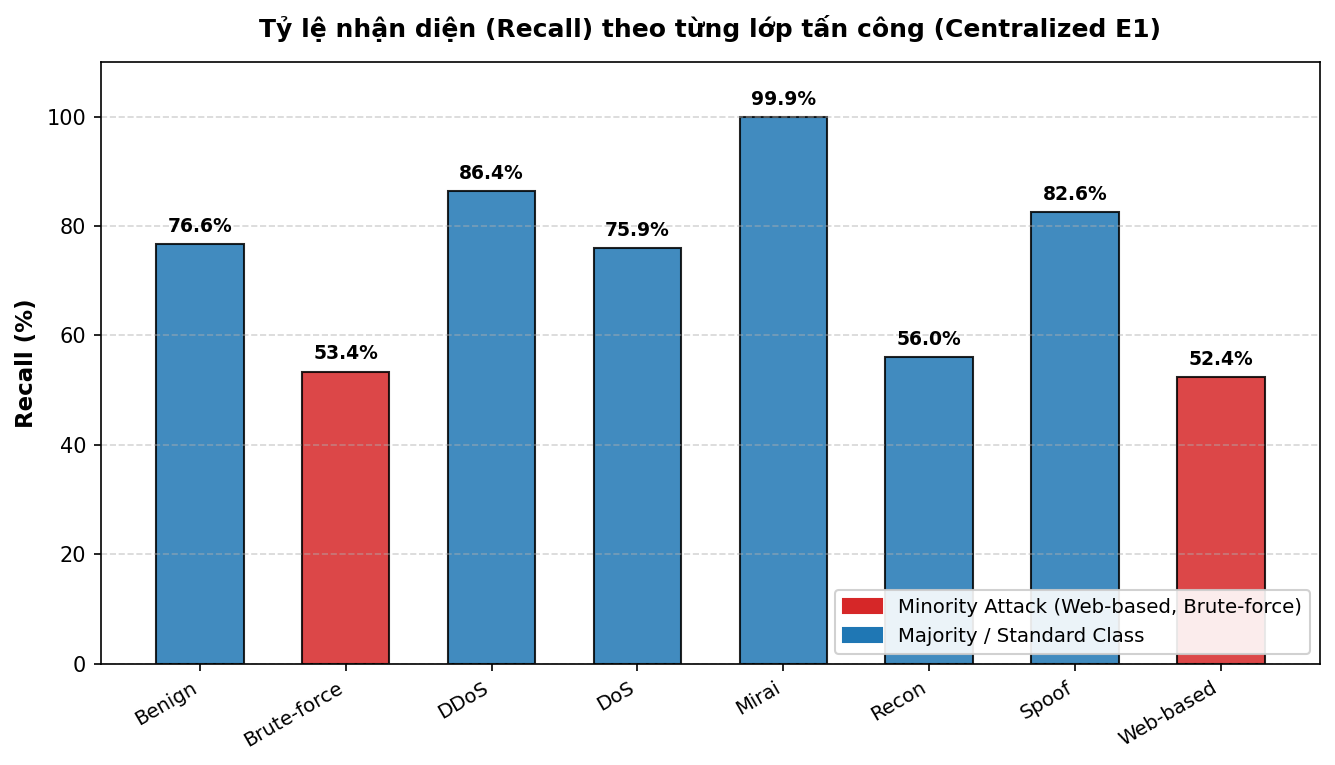
\includegraphics[width=\textwidth]{figures/recall_e1_centralized.png}
        \caption{Per-class Recall: E1 Centralized Baseline.}
        \label{fig:recall_e1_centralized}
    \end{subfigure}
    \hfill
    \begin{subfigure}[b]{0.48\textwidth}
        \centering
        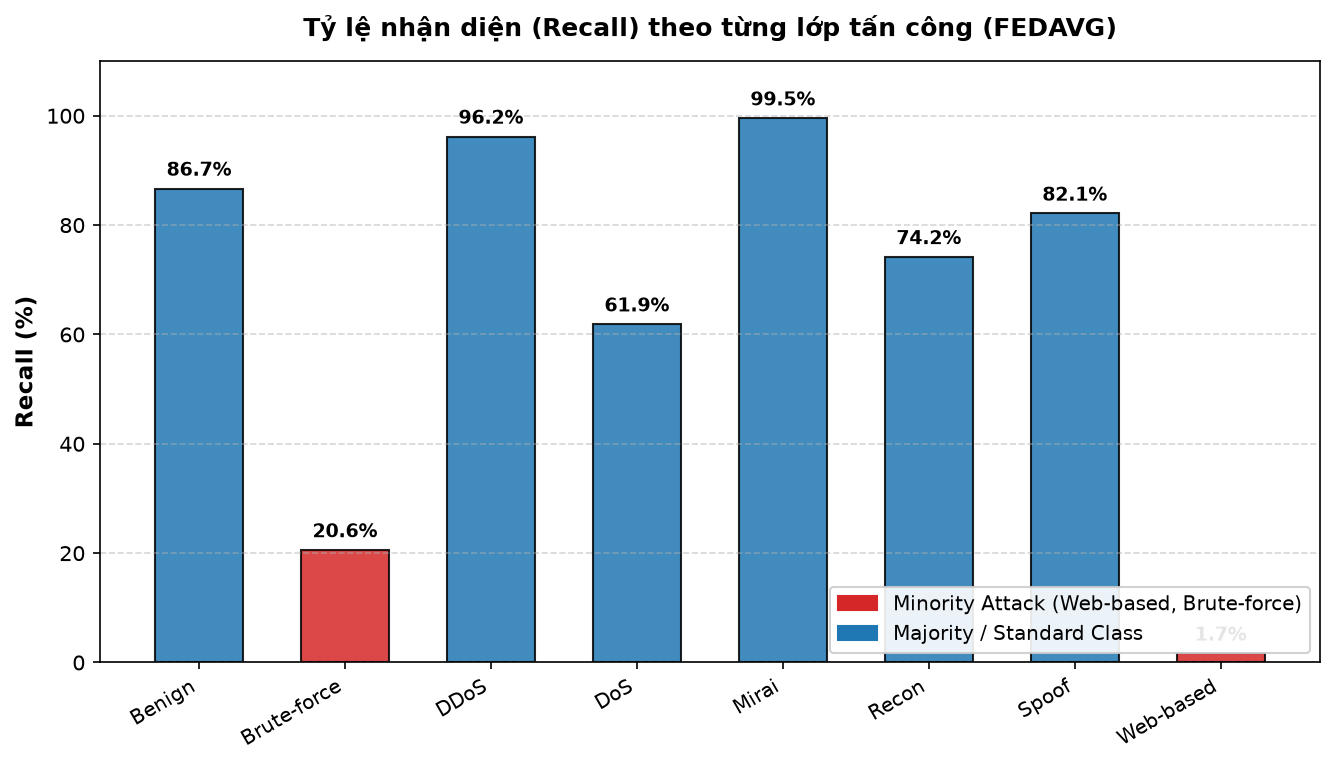
\includegraphics[width=\textwidth]{figures/recall_e2_fedavg.png}
        \caption{Per-class Recall: E2 FedAvg IID.}
        \label{fig:recall_e2_fedavg}
    \end{subfigure}
    \caption{Per-class Recall comparison demonstrating minority class collapse in federated settings.}
    \label{fig:recall_comparison}
\end{figure}

\subsection{Finding 2: Superior Detection Performance on High-Volume Infrastructure Attacks}
Bảng \ref{tab:per_class_e2} chi tiết hóa hiệu năng phân loại theo từng lớp của kịch bản E2 FedAvg trên tập kiểm định toàn cục $1,534,918$ mẫu.

\begin{table}[H]
\centering
\caption{Detailed per-class classification performance of FL-IoT-IDS (Scenario E2 FedAvg IID).}
\label{tab:per_class_e2}
\small
\begin{tabular}{l c c c r}
\toprule
\textbf{Attack Class} & \textbf{Precision (\%)} & \textbf{Recall (\%)} & \textbf{F1-score (\%)} & \textbf{Support (Test Samples)} \\
\midrule
\texttt{Mirai Botnet} & \textbf{99.85} & \textbf{99.54} & \textbf{99.70} & 63,247 \\
\texttt{DDoS Attack} & 86.88 & \textbf{96.20} & \textbf{91.30} & 576,601 \\
\texttt{Spoofing} & 89.04 & 82.12 & 85.44 & 127,981 \\
\texttt{Benign (Normal)} & 80.60 & 86.68 & 83.53 & 329,458 \\
\texttt{Reconnaissance} & 75.82 & 74.18 & 74.99 & 207,160 \\
\texttt{DoS Attack} & 86.14 & 61.86 & 72.01 & 219,103 \\
\texttt{Brute-force} & 94.60 & 20.57 & 33.79 & 3,919 \\
\texttt{Web-based} & 70.06 & \textbf{1.66} & \textbf{3.25} & 7,449 \\
\bottomrule
\end{tabular}
\end{table}

Số liệu chứng minh hệ thống đạt khả năng phòng thủ tuyệt đối trước các mối nguy hại hạ tầng nguy hiểm nhất của thế giới IoT:
\begin{itemize}
    \item \textbf{Mã độc Mirai Botnet:} Đạt F1-score $\mathbf{99.70\%}$ với tỷ lệ Recall bắt trúng lên tới $\mathbf{99.54\%}$ trên $63,247$ mẫu kiểm định.
    \item \textbf{Tấn công DDoS:} Đạt F1-score $\mathbf{91.30\%}$ và Recall $\mathbf{96.20\%}$ trên hơn nửa triệu gói tin kiểm định.
    \item \textbf{Lưu lượng Hợp lệ (Benign):} Đạt F1-score $83.53\%$ và Precision $80.60\%$, bảo đảm tỷ lệ cảnh báo giả (False Positive Rate) ở mức chấp nhận được trong vận hành mạng.
\end{itemize}

\subsection{Finding 3: Quantified Dirichlet Degradation Curve and Scalability Analysis}
\begin{itemize}
    \item \textbf{Kiểm soát độ trôi tham số (Drift L2 Norm):} Ở FedAvg, khi mức độ phân tán Non-IID tăng từ $\alpha=1.0$ lên $\alpha=0.5$, độ trôi tăng từ $10.75$ lên $13.30$ ($+23.7\%$). Ngược lại, FedProx kiểm soát trôi dạt cực kỳ nghiêm ngặt, luôn duy trì chuẩn $L_2$ dưới $0.65$ (giảm hơn $95\%$ so với FedAvg), minh chứng số hạng phạt proximal hoạt động đúng chức năng toán học của nó.
    \item \textbf{Ngưỡng gãy đổ $\alpha = 0.5$ và sụp đổ tại $\alpha = 0.1$:} Từ IID ($68.00\%$) sang $\alpha=1.0$ ($67.62\%$), hiệu năng suy giảm không đáng kể ($-0.38\%$). Tuy nhiên, khi vượt qua ngưỡng $\alpha = 0.5$, Macro-F1 bắt đầu suy giảm nhanh ($64.73\%$), và tại $\alpha = 0.1$, hệ thống rơi vào vùng suy thoái nghiêm trọng với Macro-F1 chỉ còn $43.01\%$ (mất tới gần $25\%$ hiệu năng).
    \item \textbf{Tính tuyến tính khi mở rộng quy mô ($K=5 \to 7 \to 10$):} Trong điều kiện IID, khi số lượng client tăng gấp đôi, Macro-F1 duy trì độ ổn định cao ($68.00\% \to 67.82\% \to 67.28\%$, mức biến thiên $<0.72\%$), trong khi chi phí truyền thông tích lũy tăng tuyến tính hoàn hảo ($5.30\text{ MB} \to 7.42\text{ MB} \to 10.60\text{ MB}$).
\end{itemize}

\begin{figure}[H]
    \centering
    \begin{subfigure}[b]{0.48\textwidth}
        \centering
        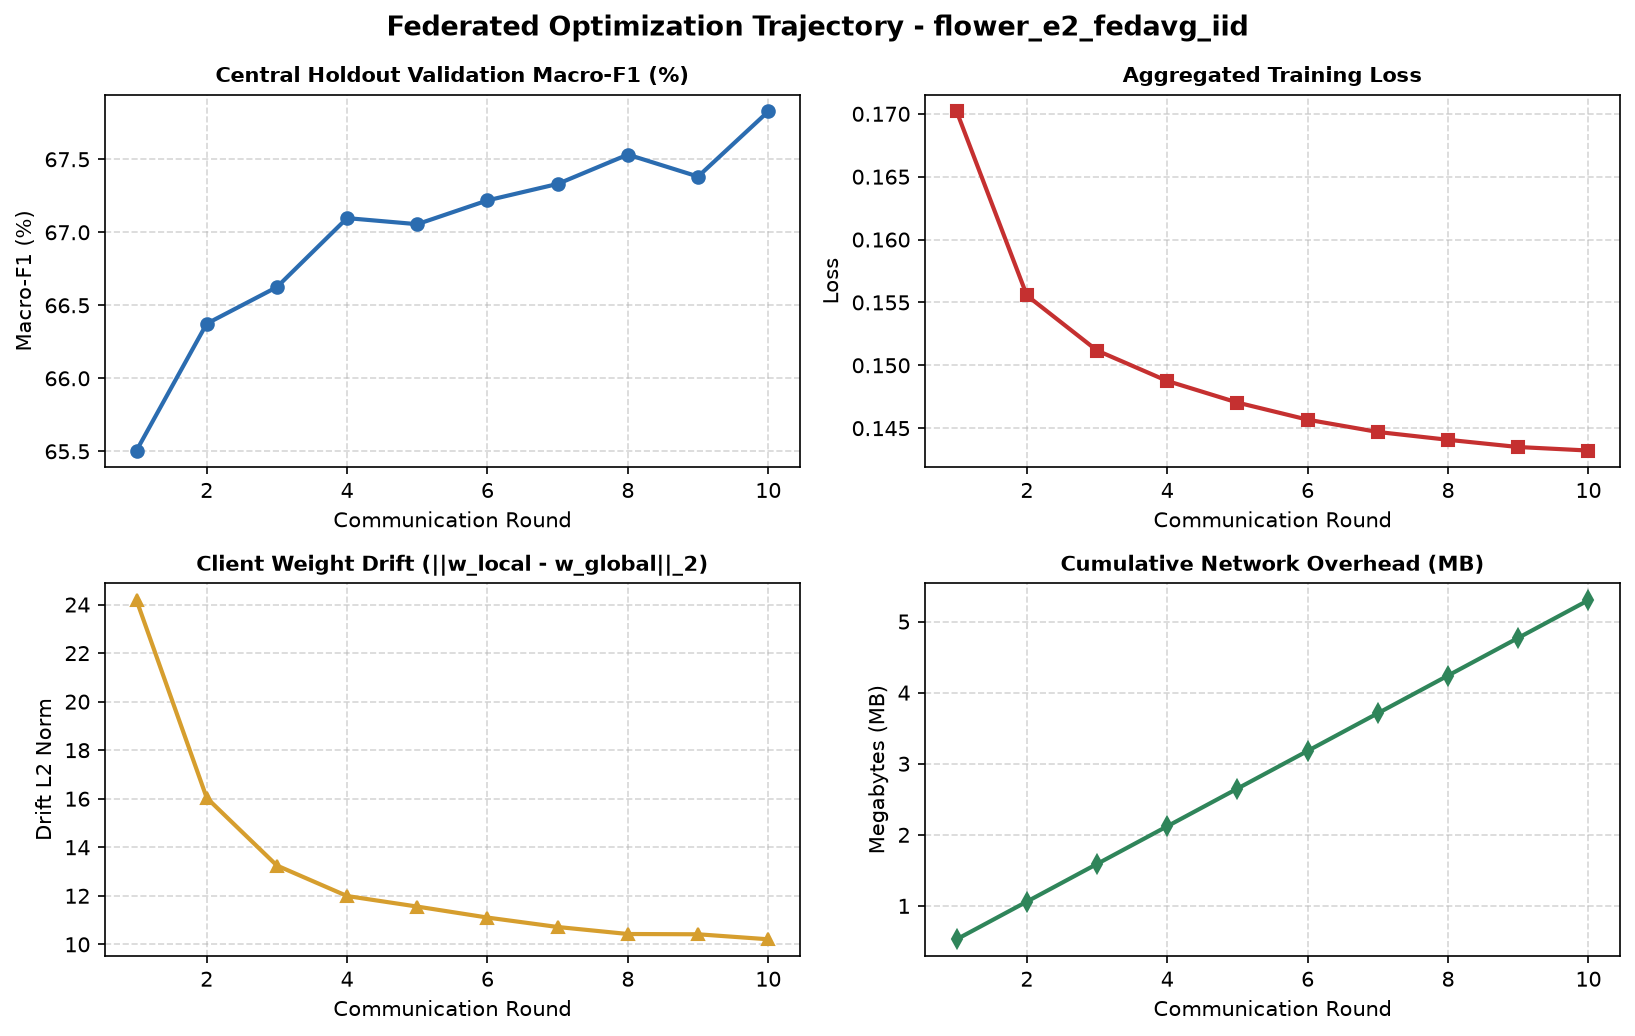
\includegraphics[width=\textwidth]{figures/conv_e2_fedavg.png}
        \caption{Convergence trajectory with $K=5$ clients (E2 FedAvg IID).}
        \label{fig:conv_e2_fedavg}
    \end{subfigure}
    \hfill
    \begin{subfigure}[b]{0.48\textwidth}
        \centering
        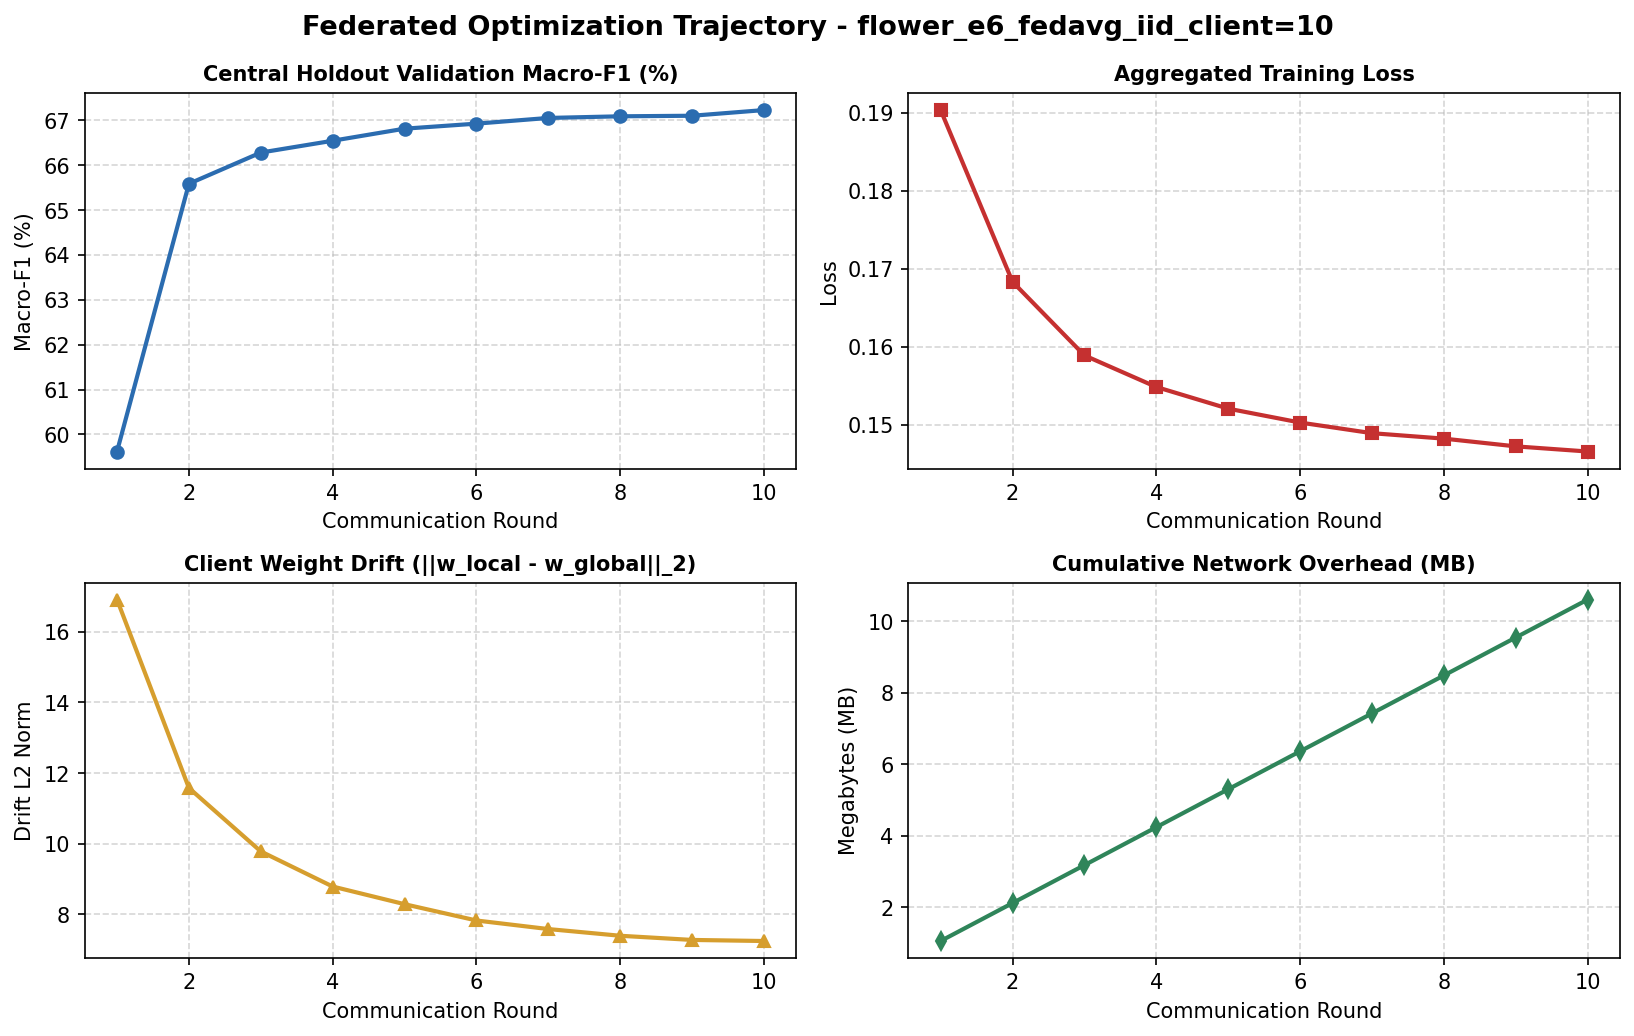
\includegraphics[width=\textwidth]{figures/conv_e6_10clients.png}
        \caption{Convergence trajectory with $K=10$ clients (E6 FedAvg IID).}
        \label{fig:conv_e6_10clients}
    \end{subfigure}
    \caption{Global Macro-F1 convergence trajectories across 10 communication rounds.}
    \label{fig:convergence_comparison}
\end{figure}

\begin{figure}[H]
    \centering
    \begin{subfigure}[b]{0.48\textwidth}
        \centering
        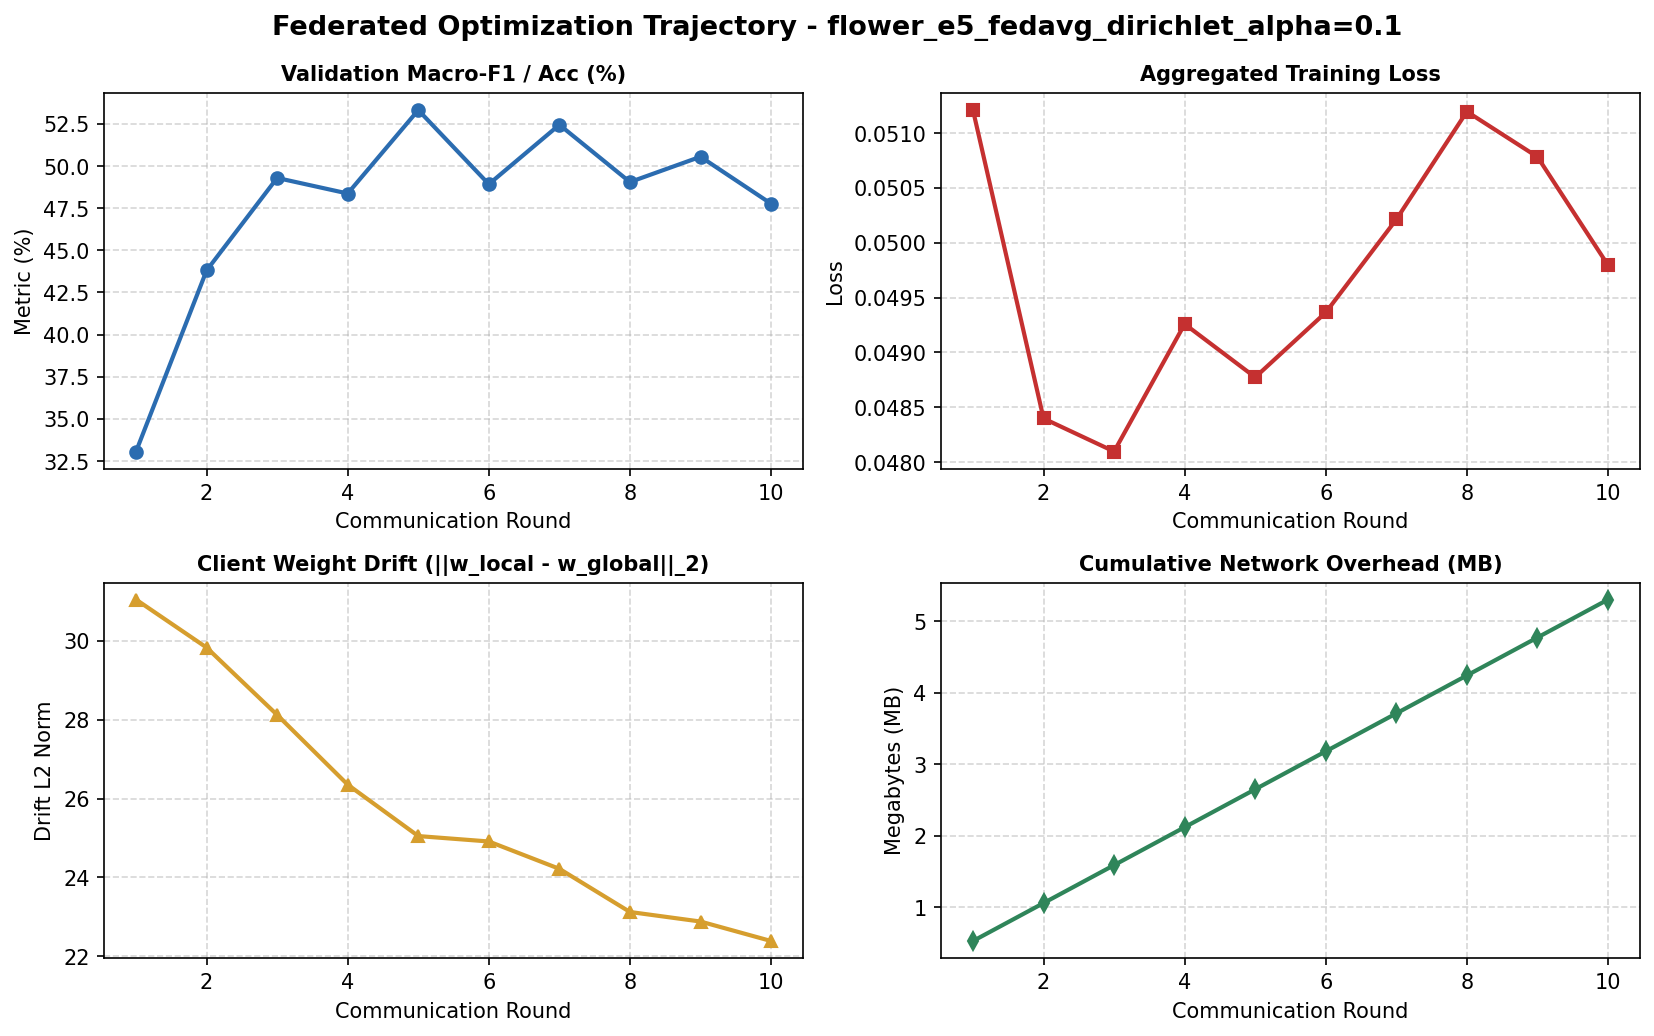
\includegraphics[width=\textwidth]{figures/conv_e5_fedavg.png}
        \caption{Convergence trajectory: E5 FedAvg ($\alpha=0.1$).}
        \label{fig:conv_e5_fedavg}
    \end{subfigure}
    \hfill
    \begin{subfigure}[b]{0.48\textwidth}
        \centering
        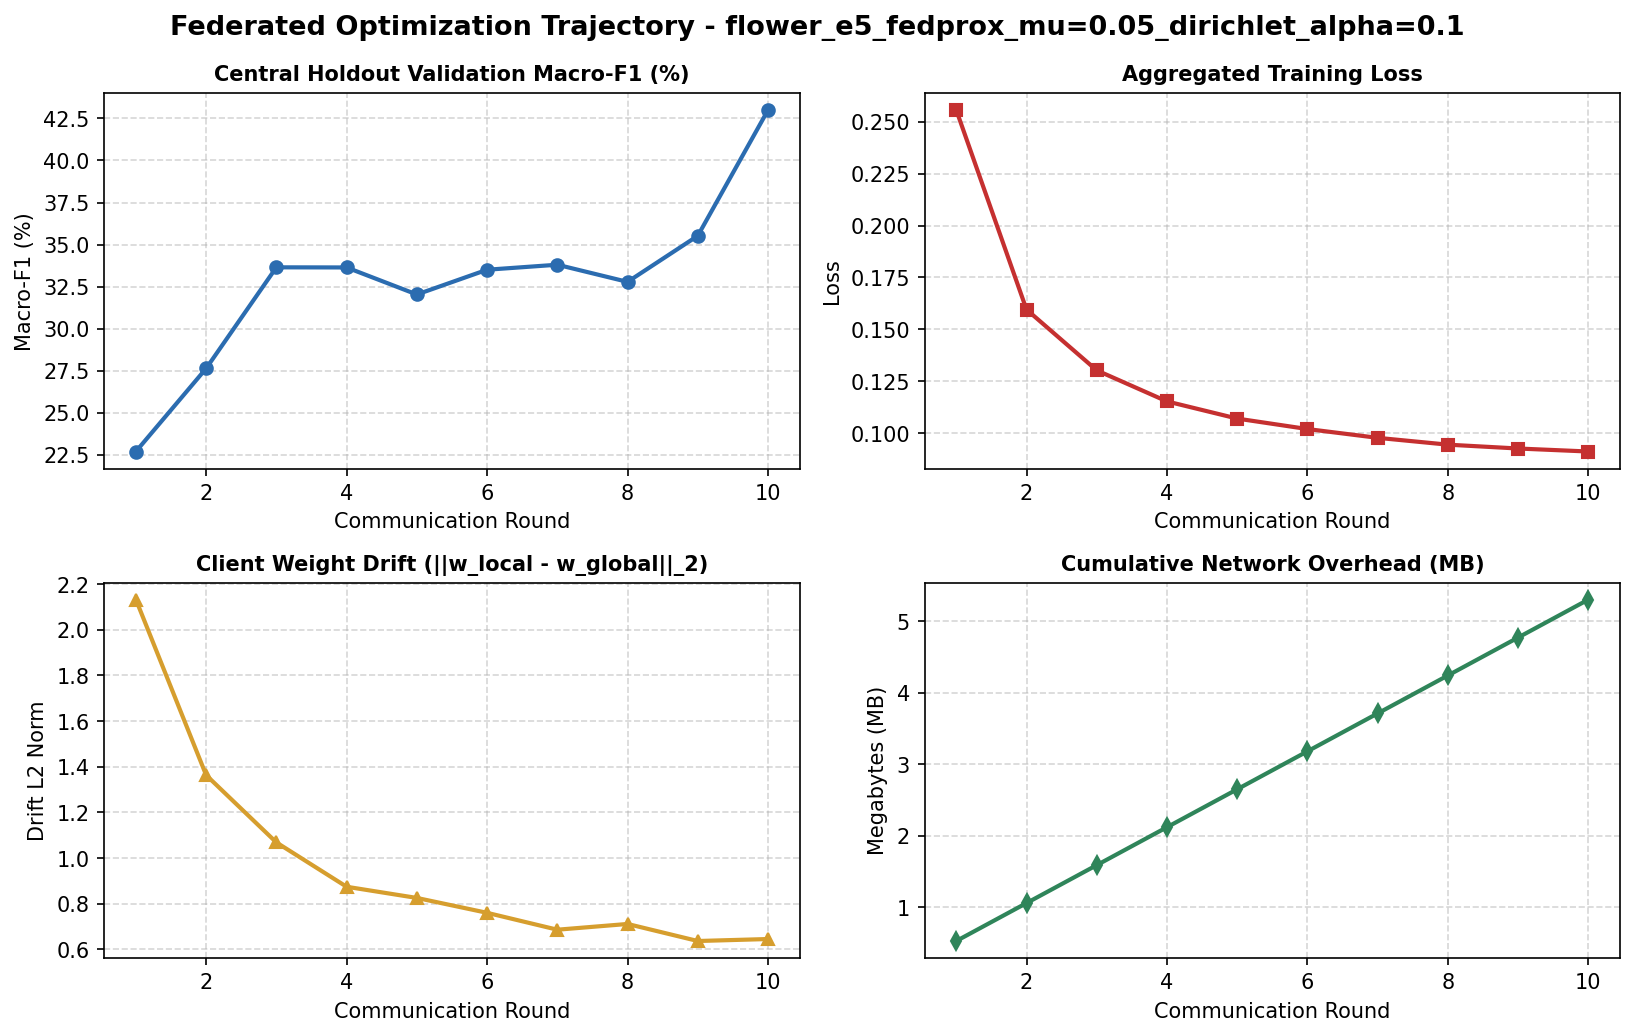
\includegraphics[width=\textwidth]{figures/conv_e5_fedprox.png}
        \caption{Convergence trajectory: E5 FedProx ($\mu=0.05, \alpha=0.1$).}
        \label{fig:conv_e5_fedprox}
    \end{subfigure}
    \caption{Comparison of optimization trajectories under extreme Non-IID skew $\alpha=0.1$.}
    \label{fig:convergence_e5_comparison}
\end{figure}

\subsection{Finding 4: The Stability-Plasticity Pareto Frontier and Proximal Sensitivity Analysis}
\label{sec:res_pareto}
Việc hoàn thành trọn vẹn kịch bản đối chứng E5 FedAvg ($\alpha=0.1$) và khảo sát sâu dải siêu tham số $\mu \in \{0.001, 0.01, 0.025, 0.05\}$ mở ra phát hiện học thuật quan trọng nhất của luận văn: xác lập đường cong biên Pareto (Pareto Frontier) giữa việc kiểm soát độ trôi dạt tham số và tính dẻo nhận diện tấn công hiếm (Hình \ref{fig:pareto_frontier}).

\begin{figure}[H]
    \centering
    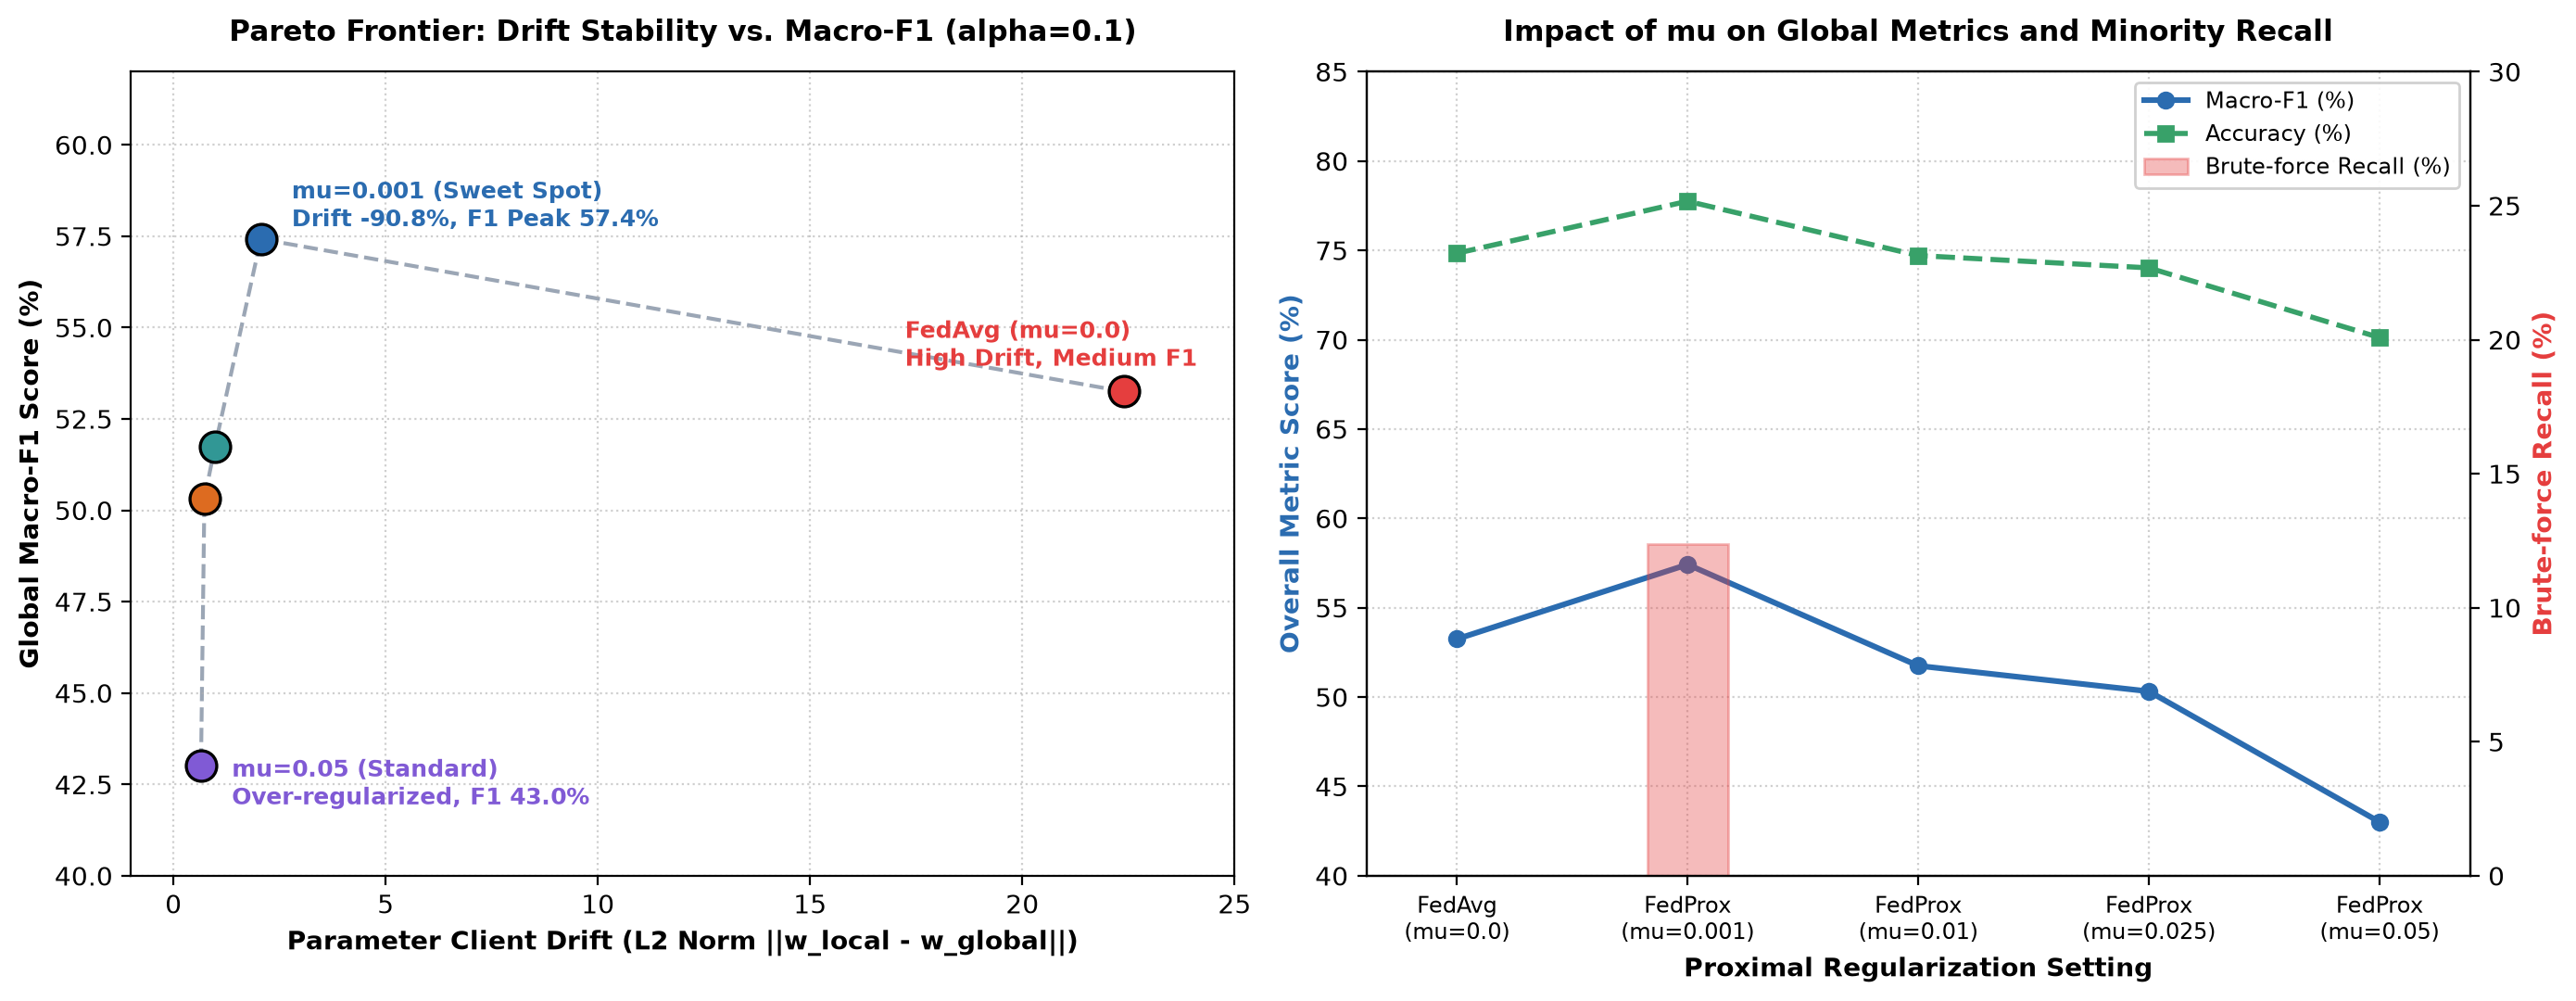
\includegraphics[width=\textwidth]{figures/pareto_frontier_e5.png}
    \caption{Empirical Pareto frontier between parameter drift stability and classification plasticity under extreme Non-IID skew ($\alpha=0.1$).}
    \label{fig:pareto_frontier}
\end{figure}

Phân tích định lượng đường cong Pareto mang lại 3 kết luận thực nghiệm cốt lõi:
\begin{enumerate}
    \item \textbf{Sự phân kỳ bùng nổ của FedAvg ($\mu=0.0$):} Khi không có số hạng phạt proximal ràng buộc, việc các client thực hiện cập nhật gradient độc lập trên các phân vùng nhãn bị phân mảnh cực đoan ($\alpha=0.1$) dẫn đến độ trôi dạt tham số $L_2$ tăng vọt lên tới $\mathbf{22.39}$ (cao gấp hơn $2$ lần so với mức $10.75$ ở $\alpha=1.0$). Mô hình toàn cục đạt Macro-F1 $53.25\%$, nhưng hoàn toàn không thể học được hai lớp tấn công thiểu số (\texttt{Web-based} và \texttt{Brute-force} đều bằng $0.00\%$) do không có cơ chế dung hòa các hướng gradient đối nghịch giữa các nút biên.
    \item \textbf{Điểm tối ưu Pareto tại $\mu = 0.001$ (The Pareto Sweet Spot):} Tại giá trị $\mu = 0.001$, lực cản proximal đủ mạnh để kiểm soát quỹ đạo tối ưu, giúp kéo giảm độ trôi dạt tham số tới $\mathbf{90.8\%}$ (từ $22.39$ xuống còn $\mathbf{2.06}$). Đồng thời, vì không bị ghìm giữ quá chặt, gradient địa phương vẫn giữ được tính dẻo để thích nghi với các mẫu tấn công hiếm: tỷ lệ Recall của \texttt{Brute-force} được giải phóng và phục hồi lên mức $\mathbf{12.38\%}$ (thay vì bị dập tắt hoàn toàn về $0.00\%$). Nhờ đó, Macro-F1 tổng thể đạt đỉnh $\mathbf{57.42\%}$, cao hơn FedAvg $+4.17\%$ và vượt trội hơn FedProx chuẩn ($\mu=0.05$) tới $\mathbf{+14.41\%}$.
    \item \textbf{Hiệu ứng quá điều hòa (Over-regularization Collapse) khi $\mu \ge 0.01$:} Khi tiếp tục tăng $\mu$ lên $0.01 \to 0.025 \to 0.05$, độ trôi tham số tiếp tục giảm nhẹ ($2.06 \to 0.98 \to 0.73 \to 0.65$), nhưng cái giá phải trả là sự suy thoái nghiêm trọng của toàn bộ mô hình:
    \begin{itemize}
        \item Lớp \texttt{Brute-force} lập tức bị dập tắt trở lại $0.00\%$.
        \item Lớp \texttt{Mirai Botnet} sụp đổ nghiêm trọng từ $80.29\%$ xuống chỉ còn $30.93\%$ tại $\mu=0.05$.
        \item Điểm Macro-F1 rơi tự do từ $57.42\%$ xuống $43.01\%$, thấp hơn cả mô hình FedAvg thông thường.
    \end{itemize}
\end{enumerate}
Kết quả này bác bỏ một cách thuyết phục giả định trong các nghiên cứu gần đây rằng việc tăng $\mu$ hoặc cố định $\mu = 0.05$ luôn có lợi cho mạng IoT Non-IID. Thực tế chứng minh rằng sự ổn định tham số trong FedProx chỉ phát huy hiệu quả khi được thiết lập ở mức cực nhỏ ($\mu \approx 10^{-3}$), còn việc lạm dụng ràng buộc proximal sẽ biến hệ thống IDS thành một bộ phân loại thiên vị tuyệt đối cho các lớp tấn công đa số.

\section{Objective Analysis of System Limitations and Defense-in-Depth Positioning}
\label{sec:res_limitations}
Dưới góc nhìn phản biện khoa học khách quan, nghiên cứu thẳng thắn nhìn nhận 4 hạn chế kỹ thuật của hệ thống prototype hiện tại:
\begin{enumerate}
    \item \textbf{Điểm mù thực tế đối với tấn công Web-based và Định vị Phòng thủ Chiều sâu (Defense-in-Depth):} Một hệ thống NIDS bỏ lọt $98\% - 99\%$ các cuộc tấn công Web-based không thể hoạt động như một giải pháp độc lập (Stand-alone Solution). Do đó, mô hình FL-IoT-IDS được định vị trong kiến trúc an ninh mạng đa tầng:
    \begin{itemize}
        \item \textit{Tầng Ứng dụng (Layer 7):} Các cuộc tấn công Web (SQL Injection, XSS) đòi hỏi giải mã và phân tích sâu nội dung payload HTTP/HTTPS, bắt buộc phải do Tường lửa ứng dụng web (WAF) hoặc Signature-based IDS (như Suricata, Snort) đảm nhiệm.
        \item \textit{Tầng Mạng/Giao vận (Layer 3/Layer 4 -- Phạm vi Đề tài):} Mô hình FL-IoT-IDS tập trung phát hiện tối ưu các cuộc tấn công lưu lượng lớn (DDoS, DoS, Botnet Mirai, Reconnaissance, Spoofing) với độ chính xác và Recall vượt trội ($>85\% - 99\%$), giải phóng tải tính toán cho các thiết bị phân tích tầng trên.
    \end{itemize}
    \item \textbf{Khoảng cách giữa mô phỏng đa tiến trình gRPC và mạng IoT vật lý:} Dù đã sử dụng giao thức socket TCP/IP gRPC thực thụ, môi trường thử nghiệm trên một máy chủ chưa thể tái hiện đầy đủ các yếu tố ngẫu nhiên của sóng vô tuyến: mất gói tin (packet loss), trễ biến thiên (jitter), thiết bị ngắt kết nối đột ngột (client dropouts), và sự không đồng nhất về phần cứng (thiết bị chạy nhanh, thiết bị chạy chậm -- Straggler problem).
    \item \textbf{Thiên kiến tập dữ liệu đơn (Single-Dataset Bias):} Toàn bộ các kết luận thực nghiệm mới được kiểm chứng trên CICIoT2023. Để nâng cao tính tổng quát hóa, mô hình cần được thử nghiệm chéo trên các tập dữ liệu khác như Edge-IIoTset hoặc TON\_IoT.
    \item \textbf{Nguy cơ từ tấn công đầu độc trọng số (No Byzantine Robustness):} FedAvg và FedProx mặc định toàn bộ các nút tham gia đều trung thực. Trong thực tế, chỉ cần 1 client bị chiếm quyền điều khiển và gửi các vector trọng số độc hại (Poisoning/Backdoor attack), mô hình toàn cục có thể bị vô hiệu hóa hoàn toàn \cite{blanchard2017machine, yin2018byzantine}. Khung mã nguồn của đề tài đã chuẩn bị sẵn các mô-đun mở rộng cho \texttt{FedMedian} và \texttt{FedTrimmedMean} để nghiên cứu sâu hơn.
\end{enumerate}
